\subsection{UC1: Utilizzo editor grafico}
\hypertarget{UC1}{} 
\begin{figure} [H]
	\centering
	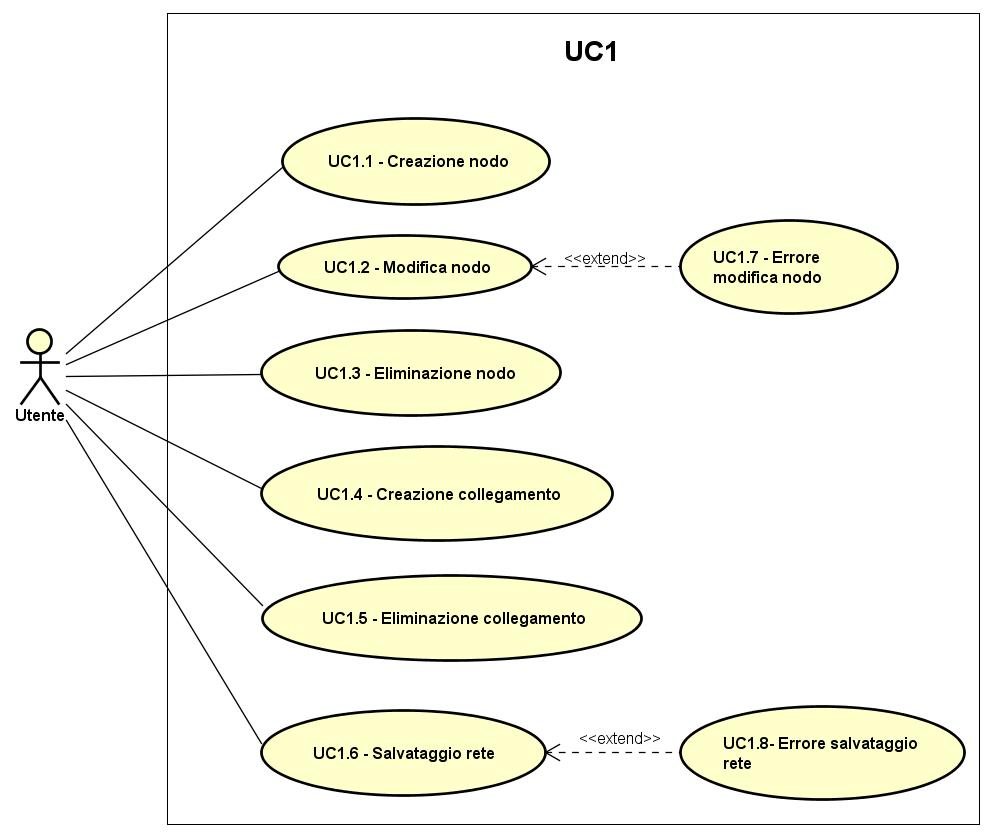
\includegraphics[scale=0.45]{Img/UC1} 
	\caption{UC1 - Utilizzo editor grafico} \label{} 
\end{figure} 
\begin{itemize} 
	\item{\textbf{Attori primari}: Utente;}
	\item{\textbf{Scopo e descrizione}: l'attore vuole utilizzare l'editor grafico ai fini di realizzare facilmente tramite interfaccia grafica un'apposita rete Bayesiana, o modificarne una già esistente;} 
	\item{\textbf{Precondizione}: l'editor grafico è stato caricato correttamente ed è pronto all'uso;} 
	\item{\textbf{Flusso base degli eventi}: 
		\begin{itemize} 
			\item{L'attore crea uno o più nodi (UC1.1);} 
			\item{L'attore modifica i parametri dei nodi impostati inizialmente con valori di default(UC1.2);} 
			\item{L'attore può eliminare o modificare nuovamente determinati nodi (UC1.3, UC1.2)}; 
			\item{L'attore crea un collegamento tra nodi (UC1.4);} 
			\item{L'attore può eliminare determinati collegamenti in eccesso (UC1.5);} 
			\item{L'attore effettua il salvataggio della rete su un apposito file (UC1.6).} 
		\end{itemize} 
	} 
	\item{\textbf{Postcondizione}: il sistema ha ottenuto le informazioni sulle operazioni che l'attore desidera eseguire e le ha eseguite.} 
\end{itemize} 
\subsection{UC1.1: Creazione di un nodo}
\hypertarget{UC1.1}{}  
\begin{figure} [H]
	\centering
	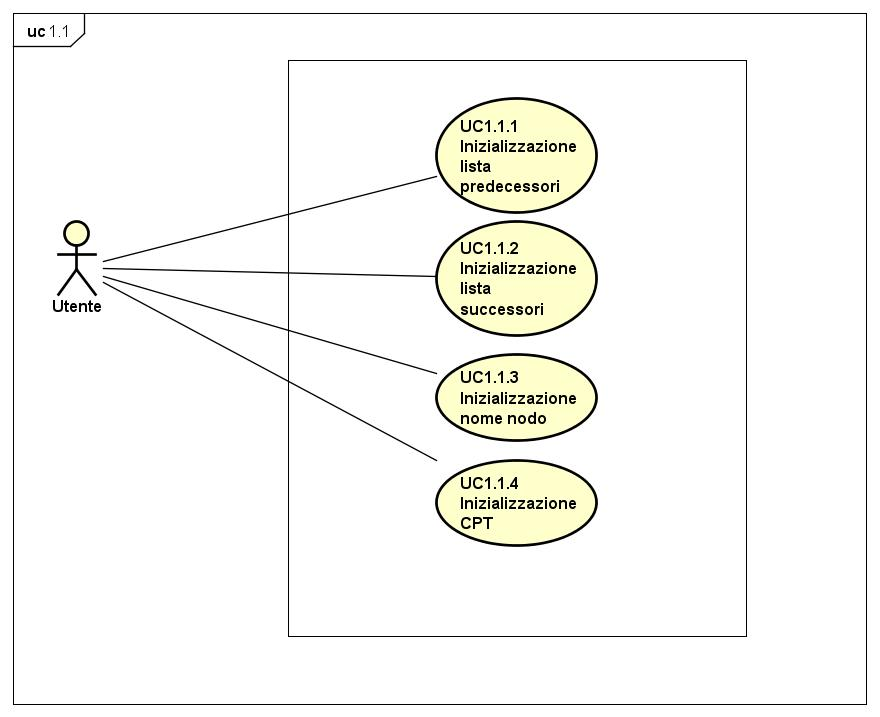
\includegraphics[scale=0.45]{Img/UC1-1} 
	\caption{UC1.1 - Creazione di un nodo} \label{} 
\end{figure} 
\begin{itemize} 
	\item{\textbf{Attori primari}: Utente;} 
	\item{\textbf{Scopo e descrizione}: l'attore desidera creare un nodo della rete Bayesiana. Un nodo della rete Bayesiana è composto da quattro componenti: 
		\begin{itemize} 
			\item{Il nome del nodo;} 
			\item{Una \gl{CPT};} 
			\item{La lista dei predecessori;} 
			\item{La lista dei successori.} 
		\end{itemize} 
		Al momento della creazione del nodo tutte le componenti vengono inizializzate con valori di default;} 
	\item{\textbf{Precondizione}: l'attore ha indicato al sistema di voler inserire un nodo all'interno della rete Bayesiana;} 
	\item{\textbf{Flusso base degli eventi}: } 
	\begin{itemize} 
		\item{Inizializzazione lista predecessori(UC1.1.1);} 
		\item{Inizializzazione lista successori(UC1.1.2);} 
		\item{Inizializzazione nome nodo (UC1.1.3);} 
		\item{Inizializzazione CPT(UC1.1.4).} 
	\end{itemize} 
	\item{\textbf{Postcondizione}: il sistema ha creato un nodo le cui componenti sono state tutte inizializzate correttamente con valori di default.} 
\end{itemize} 
\subsection{UC1.1.1: Inizializzazione lista predecessori} 
\hypertarget{UC1.1.1}{} 
\begin{itemize} 
	\item{\textbf{Attori primari}: Utente;} 
	\item{\textbf{Scopo e descrizione}: un nodo al momento della sua creazione nasce completamente distaccato dalla rete, di conseguenza non possiede alcun predecessore e la relativa lista dovrà essere vuota;} 
	\item{\textbf{Precondizione}: l'attore ha indicato al sistema di voler inserire un nodo all'interno della rete Bayesiana;} 
	\item{\textbf{Postcondizione}: l'inizializzazione della lista di predecessori è stata completata correttamente.} 
\end{itemize} 
\subsection{UC1.1.2: Inizializzazione lista successori} 
\hypertarget{UC1.1.2}{} 
\begin{itemize} 
	\item{\textbf{Attori primari}: Utente;} 
	\item{\textbf{Scopo e descrizione}: un nodo al momento della sua creazione nasce completamente distaccato dalla rete, di conseguenza non possiede alcun successore e la relativa lista dovrà essere vuota;} 
	\item{\textbf{Precondizione}: l'attore ha indicato al sistema di voler inserire un nodo all'interno della rete Bayesiana;} 
	\item{\textbf{Postcondizione}: l'inizializzazione della lista di successori è stata completata correttamente.} 
\end{itemize} 
\subsection{UC1.1.3: Inizializzazione nome nodo}
\hypertarget{UC1.1.3}{}  
\begin{itemize} 
	\item{\textbf{Attori primari}: Utente;} 
	\item{\textbf{Scopo e descrizione}: il nome del nodo viene inizializzato con un valore di default composto dalla stringa "Nodo" seguita da un numero progressivo che parte da 1 e viene incrementato ad ogni creazione di un nodo;} 
	\item{\textbf{Precondizione}: l'attore ha effettuato la creazione di un nuovo nodo della rete;} 
	\item{\textbf{Postcondizione}: l'inizializzazione del titolo del nodo è stata completata correttamente.} 
\end{itemize} 

\subsection{UC1.1.4: Inizializzazione CPT} 
\hypertarget{UC1.1.4}{} 
\begin{figure} [H]
	\centering
	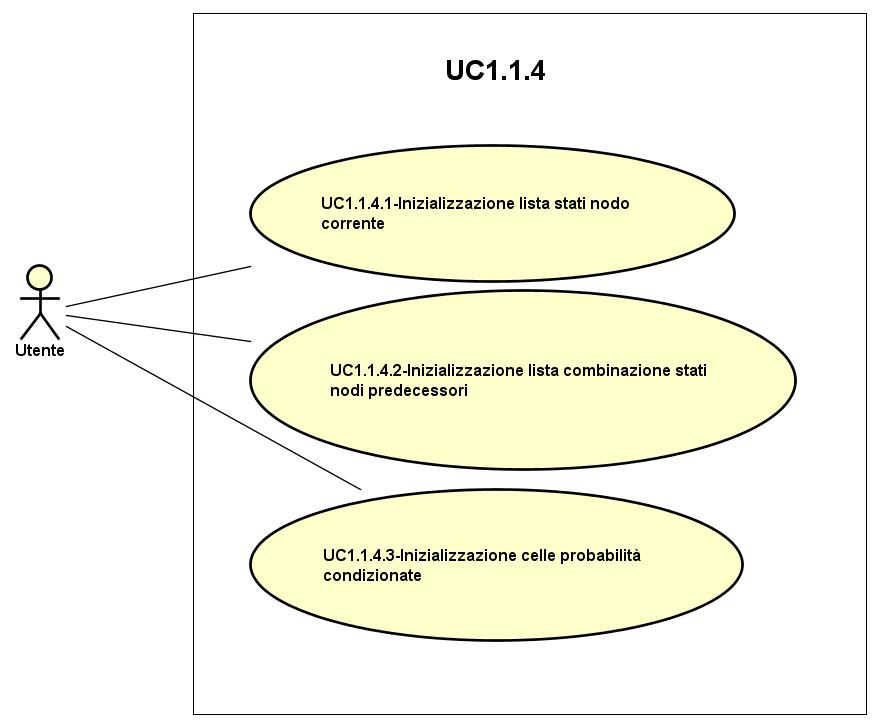
\includegraphics[scale=0.45]{Img/UC1-1-4} 
	\caption{UC1.1.4 - Inizializzazione CPT} \label{} 
\end{figure} 
\begin{itemize} 
	\item{\textbf{Attori primari}: Utente;} 
	\item{\textbf{Scopo e descrizione}: una CPT è composta principalmente da tre componenti: 
		\begin{itemize} 
			\item{La lista dei possibili stati in cui il nodo corrente può risiedere;} 
			\item{La lista di tutte le combinazioni esistenti di tutti i possibili stati dei nodi predecessori;} 
			\item{La tabella delle probabilità vera e propria, in cui ogni cella è identificata da una coppia di elementi delle liste dei due punti precedenti.} 
		\end{itemize} 			
		Ogni punto deve essere inizializzato correttamente tramite appositi valori di default;
	} 
	\item{\textbf{Precondizione}: l'attore ha effettuato la creazione di un nuovo nodo della rete;} 
	\item{\textbf{Flusso base degli eventi}: } 
	\begin{itemize} 
		\item{Inizializzazione lista stati nodo corrente(UC1.1.4.1);} 
		\item{Inizializzazione lista combinazione stati nodi predecessori(UC1.1.4.2);} 
		\item{Inizializzazione celle tabella probabilità condizionate (UC1.1.4.3).} 
	\end{itemize} 
	\item{\textbf{Postcondizione}: l'inizializzazione della CPT è stata completata correttamente.} 
\end{itemize} 
\subsection{UC1.1.4.1: Inizializzazione lista stati nodo corrente} 
\hypertarget{UC1.1.4.1}{} 
\begin{itemize} 
	\item{\textbf{Attori primari}: Utente;} 
	\item{\textbf{Scopo e descrizione}: la lista degli stati del nodo corrente viene inizializzata di default con due stati distinti. Ad ogni stato del nodo corrente è associato un nome ed un intervallo di valori, anche essi dovranno essere inizializzati con valori di default;} 
	\item{\textbf{Precondizione}: l'attore ha effettuato la creazione di un nuovo nodo della rete;} 
	\item{\textbf{Postcondizione}: l'inizializzazione della lista di stati del nodo corrente è stata completata correttamente.} 
\end{itemize} 
\subsection{UC1.1.4.2: Inizializzazione lista combinazioni stati nodi predecessori} 
\hypertarget{UC1.1.4.2}{} 
\begin{itemize} 
	\item{\textbf{Attori primari}: Utente;} 
	\item{\textbf{Scopo e descrizione}: un nodo al momento della sua creazione nasce privo di predecessori e successori, di conseguenza la lista di predecessori dovrà essere vuota;} 
	\item{\textbf{Precondizione}: l'attore ha effettuato la creazione di un nuovo nodo della rete;} 
	\item{\textbf{Postcondizione}: l'inizializzazione della lista delle possibili combinazioni di stati dei nodi predecessori è stata completata correttamente.} 
\end{itemize} 
\subsection{UC1.1.4.3: Inizializzazione celle tabella probabilità condizionate} 
\hypertarget{UC1.1.4.3}{} 
\begin{itemize} 
	\item{\textbf{Attori primari}: Utente;} 
	\item{\textbf{Scopo e descrizione}: prendendo in considerazione i sottocasi UC1.1.4.1 e UC1.1.4.2 si può affermare che la CPT di un nodo al momento della sua creazione possiede solamente due celle. Entrambe verranno inizializzate con il valore 50\%;} 
	\item{\textbf{Precondizione}: l'attore ha effettuato la creazione di un nuovo nodo della rete;} 
	\item{\textbf{Postcondizione}: l'inizializzazione delle celle della tabella delle probabilità condizionate è stata completata correttamente.} 
\end{itemize} 
\subsection{UC1.2: Modifica nodo} 
\hypertarget{UC1.2}{} 
\begin{figure} [H]
	\centering
	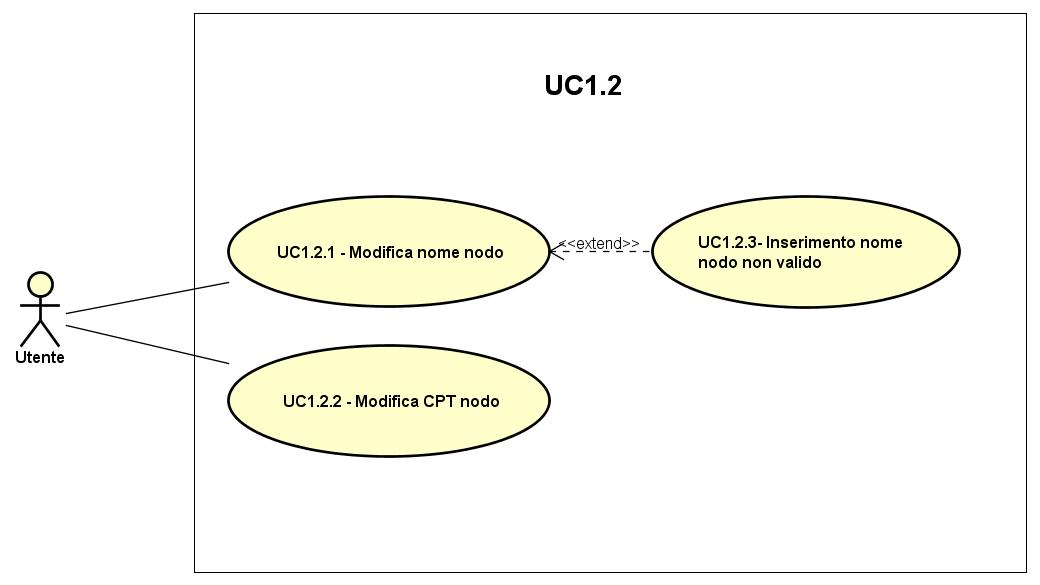
\includegraphics[scale=0.45]{Img/UC1-2} 
	\caption{UC1.2 - Modifica nodo} \label{} 
\end{figure} 
\begin{itemize} 
	\item{\textbf{Attori primari}: Utente;} 
	\item{\textbf{Scopo e descrizione}: l'attore desidera modificare il valore di uno o più parametri di un nodo della rete Bayesiana;} 
	\item{\textbf{Precondizione}: l'attore ha indicato il nodo su cui desidera effettuare l'operazione di modifica;} 
	\item{\textbf{Flusso base degli eventi}: } 
	\begin{itemize} 
		\item{L'attore può modificare il nome del nodo(UC1.2.1);} 
		\item{L'attore può modificare la CPT associata al nodo(UC1.2.2).} 		
	\end{itemize} 
	\item{\textbf{Postcondizione}: l'attore ha indicato quali parametri del nodo desidera modificare, come devono essere modificati e sono stati aggiornati correttamente;} 
	\item{\textbf{Estensioni}:} 
	\begin{itemize} 
		\item{Nel caso in cui l'attore modifichi gli attributi del nodo con valori non validi, il nodo e tutti i collegamenti ad esso associati non verranno considerati come facenti parte della rete.} 
	\end{itemize} 
\end{itemize} 
\subsection{UC1.2.1: Modifica nome nodo} 
\hypertarget{UC1.2.1}{} 
\begin{itemize} 
	\item{\textbf{Attori primari}: Utente;} 
	\item{\textbf{Scopo e descrizione}: l'attore desidera modificare il nome di uno specifico nodo;} 
	\item{\textbf{Precondizione}: l'attore ha indicato al sistema di volere modificare il nome di uno specifico nodo;} 
	\item{\textbf{Postcondizione}: il nome del nodo è stato aggiornato correttamente.} 
\end{itemize} 
\subsection{UC1.2.2: Modifica CPT associata al nodo} 
\hypertarget{UC1.2.2}{} 
\begin{figure} [H]
	\centering
	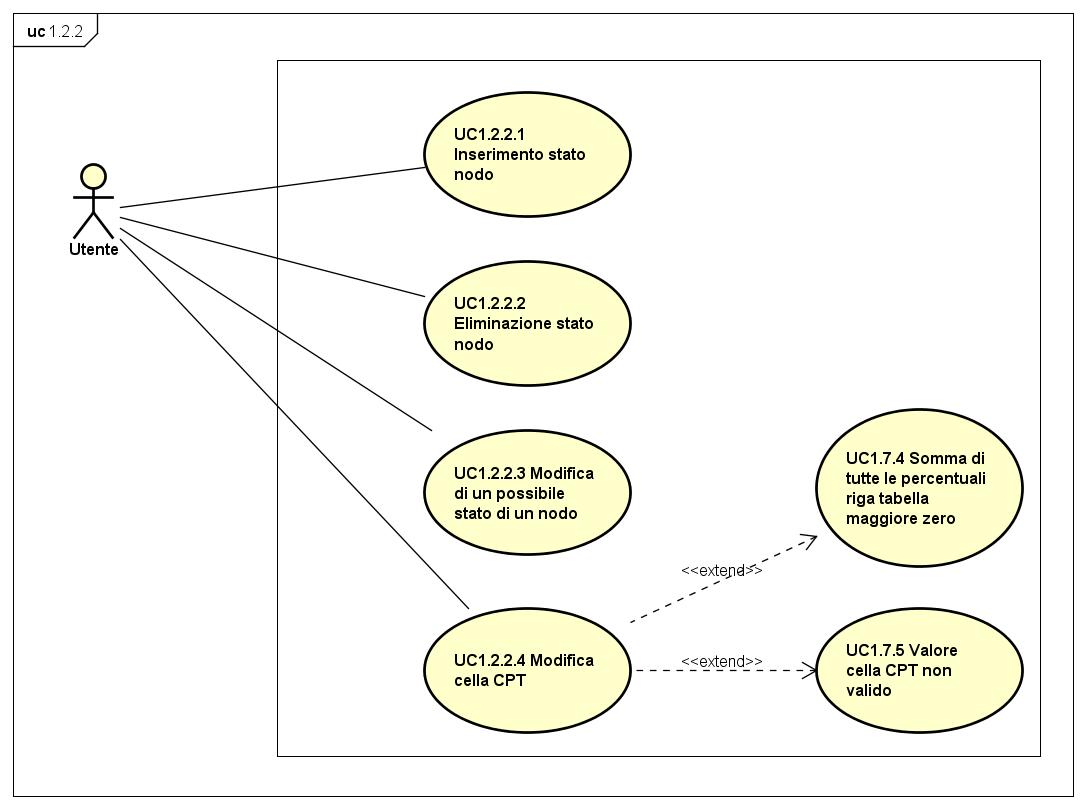
\includegraphics[scale=0.45]{Img/UC1-2-2} 
	\caption{UC1.2.2 - Modifica CPT associata al nodo} \label{} 
\end{figure} 
\begin{itemize} 
	\item{\textbf{Attori primari}: Utente;} 
	\item{\textbf{Scopo e descrizione}: l'attore desidera modificare la CPT associata al nodo. Una CPT è composta principalmente da tre componenti: 
		\begin{itemize} 
			\item{La lista dei possibili stati in cui il nodo corrente può risiedere;} 
			\item{La lista di tutte le combinazioni esistenti di tutti i possibili stati dei nodi predecessori;} 
			\item{La tabella delle probabilità vera e propria, in cui ogni cella è identificata da una coppia di elementi delle liste dei due punti precedenti.} 
		\end{itemize} 
		Questo caso d'uso si concentra principalmente sulla modifica della prima e dell'ultima componente. L'interazione dell'attore con la seconda componente verrà trattata nei casi d'uso UC1.3 e UC1.4;
	} 
	\item{\textbf{Precondizione}: l'attore ha indicato al sistema quale operazioni vuole effettuare sulla CPT di uno specifico nodo;} 
	\item{\textbf{Flusso base degli eventi}: } 
	\begin{itemize} 
		\item{L'attore può aggiungere uno stato al nodo corrente;} 
		\item{L'attore può rimuovere uno stato dal nodo corrente;} 
		\item{L'attore può modificare gli attributi associati ad uno stato del nodo corrente;} 
		\item{L'attore può modificare la probabilità contenuta in una cella della CPT.} 
	\end{itemize} 
	\item{\textbf{Postcondizione}: le operazioni richieste sono state eseguite e la CPT del nodo indicato è stata aggiornata correttamente.} 
\end{itemize} 
\subsection{UC1.2.2.1: Inserimento stato nodo} 
\hypertarget{UC1.2.2.1}{} 
\begin{itemize} 
	\item{\textbf{Attori primari}: Utente;} 
	\item{\textbf{Scopo e descrizione}: l'attore desidera creare un nuovo stato associato al nodo corrente da inserire all'interno della CPT;} 
	\item{\textbf{Precondizione}: l'attore ha indicato di volere inserire uno stato all'interno della CPT del nodo corrente;} 
	\item{\textbf{Postcondizione}: lo stato è stato inserito correttamente ed i suoi parametri sono stati inizializzati con valori di default.} 
\end{itemize} 
\subsection{UC1.2.2.2: Eliminazione stato nodo} 
\hypertarget{UC1.2.2.2}{} 
\begin{itemize} 
	\item{\textbf{Attori primari}: Utente;} 
	\item{\textbf{Scopo e descrizione}: l'attore desidera eliminare uno stato associato alla CPT del nodo corrente;} 
	\item{\textbf{Precondizione}: l'attore ha indicato quale stato vuole eliminare;} 
	\item{\textbf{Postcondizione}: lo stato è stato eliminato correttamente assieme a tutte le celle della tabella ad esso associate.} 
\end{itemize} 
\subsection{UC1.2.2.3: Modifica di un possibile stato di un nodo} 
\hypertarget{UC1.2.2.3}{} 
\begin{figure} [H]
	\centering
	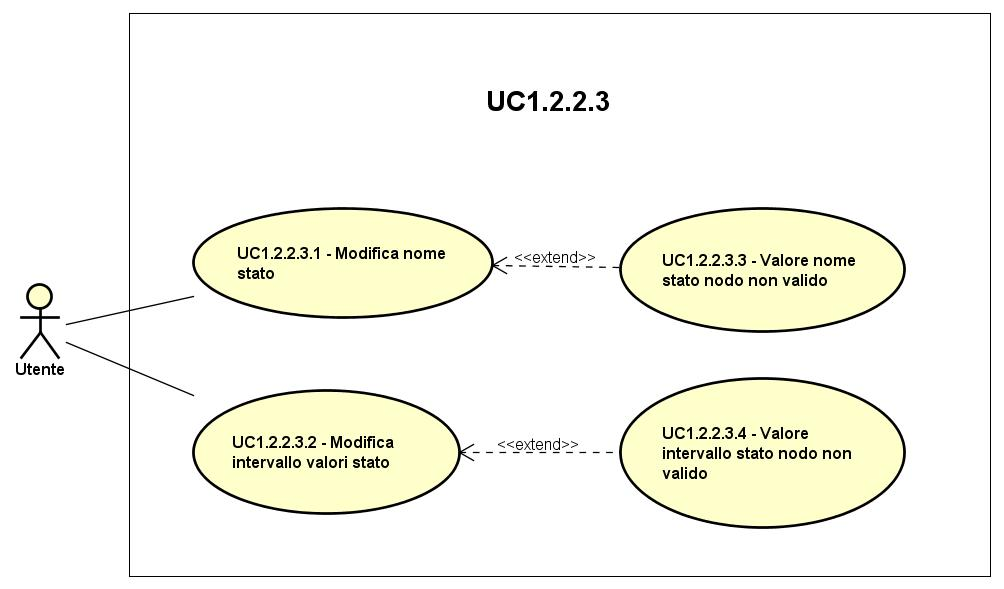
\includegraphics[scale=0.45]{Img/UC1-2-2-3} 
	\caption{UC1.2.2.3 - Modifica di un possibile stato di un nodo} \label{} 
\end{figure} 
\begin{itemize} 
	\item{\textbf{Attori primari}: Utente;} 
	\item{\textbf{Scopo e descrizione}: uno stato associato alla CPT di un nodo è composto da due componenti: un nome ed un intervallo di valori. L'attore può effettuare operazioni di modifica su entrambe le componenti;} 
	\item{\textbf{Precondizione}: l'attore ha indicato quale stato vuole modificare e come vuole modificarlo;} 
	\item{\textbf{Flusso base degli eventi}: 
		\begin{itemize} 
			\item{L'attore può modificare il nome dello stato;} 
			\item{L'attore può modificare il range di valori dello stato.} 
		\end{itemize} 			
	} 
	\item{\textbf{Postcondizione}: lo stato è stato modificato correttamente come richiesto dall'attore. Eventuali errori causati dall'inserimento di valori non validi sono stati gestiti correttamente e segnalati all'attore.} 
\end{itemize} 
\subsection{UC1.2.2.3.1: Modifica nome stato} 
\hypertarget{UC1.2.2.3.1}{} 
\begin{itemize} 
	\item{\textbf{Attori primari}: Utente;} 
	\item{\textbf{Scopo e descrizione}: l'attore desidera modificare il nome di uno stato associato alla CPT di un nodo;} 
	\item{\textbf{Precondizione}: l'attore ha indicato di volere modificare il nome di uno stato;} 
	\item{\textbf{Postcondizione}: il nome dello stato è stato aggiornato correttamente. Eventuali errori causati dall'inserimento di valori non validi sono stati gestiti correttamente e segnalati all'attore;}
	\item{\textbf{Estensioni}:
		\begin{itemize}
			\item{Valore nome stato nodo non valido (UC1.2.2.3.3)}.
		\end{itemize}
	}
\end{itemize} 
\subsection{UC1.2.2.3.2: Modifica intervallo valori stato} 
\hypertarget{UC1.2.2.3.2}{} 
\begin{itemize} 
	\item{\textbf{Attori primari}: Utente;} 
	\item{\textbf{Scopo e descrizione}: l'attore desidera modificare l'intervallo di valori associato ad uno stato;} 
	\item{\textbf{Precondizione}: l'attore ha indicato che vuole modificare l'intervallo di valori di uno stato;} 
	\item{\textbf{Postcondizione}: l'intervallo di valori è stato aggiornato correttamente come richiesto dall'attore. Eventuali errori causati dall'inserimento di valori non validi sono stati gestiti correttamente e segnalati all'attore;}
	\item{\textbf{Estensioni}:
		\begin{itemize}
			\item{Valore intervallo stato nodo non valido (UC1.2.2.3.4).}
		\end{itemize}
	}
\end{itemize}
\subsection{UC1.2.2.3.3: Valore nome stato nodo non valido} 
\hypertarget{UC1.2.2.3.3}{} 
\begin{itemize} 
	\item{\textbf{Attori primari}: Utente;} 
	\item{\textbf{Scopo e descrizione}:l'attore ha modificato il nome di uno stato di un nodo con un valore non valido. Le principali cause d'errore possono essere l'inserimento di una stringa vuota od il nome di uno stato già esistente all'interno dello stesso nodo;} 
	\item{\textbf{Precondizione}: l'attore ha modificato il nome di uno stato di un nodo;} 
	\item{\textbf{Postcondizione}: l'attore viene informato della causa d'errore ed il nome dello stato viene ripristinato al valore precedente.} 
\end{itemize}
\subsection{UC1.2.3.3.4: Valori dell'intervallo di uno stato di un nodo non validi} 
\hypertarget{UC1.2.2.3.4}{} 
\begin{itemize} 
	\item{\textbf{Attori primari}: Utente;} 
	\item{\textbf{Scopo e descrizione}: l'attore ha modificato l'intervallo di valori associato ad uno stato di un nodo con dei valori non validi. La principale causa d'errore può essere l'inserimento di un limite inferiore maggiore rispetto al limite superiore o viceversa;} 
	\item{\textbf{Precondizione}: l'attore ha modificato l'intervallo di valori associato ad uno stato di un nodo;} 
	\item{\textbf{Postcondizione}: l'attore viene informato dell'errore, il nodo e tutti i collegamenti ad esso associati vengono temporaneamente disattivati dalla rete fintanto che l'errore non viene risolto.} 
\end{itemize}
\subsection{UC1.2.2.4: Modifica cella CPT} 
\hypertarget{UC1.2.2.4}{} 
\begin{itemize} 
	\item{\textbf{Attori primari}: Utente;} 
	\item{\textbf{Scopo e descrizione}: l'attore desidera modificare la probabilità contenuta in una cella della CPT;} 
	\item{\textbf{Precondizione}: l'attore ha indicato quale cella vuole modificare e con quale valore vuole sostituire quello corrente;} 
	\item{\textbf{Postcondizione}: il valore contenuto all'interno della cella è stato aggiornato correttamente. Eventuali errori causati dall'inserimento di valori non validi sono stati gestiti correttamente e segnalati all'attore;}
	\item{\textbf{Estensioni}:
		\begin{itemize}
			\item{Somma percentuale CPT non valida (UC1.2.2.5);}
			\item{Valore cella CPT non valido (UC1.2.2.6).}
		\end{itemize}
	}
\end{itemize}
\subsection{UC1.2.2.5: Somma percentuali CPT non valida} 
\hypertarget{UC1.2.2.5}{} 
\begin{itemize} 
	\item{\textbf{Attori primari}: Utente;} 
	\item{\textbf{Scopo e descrizione}: per ogni possibile combinazione esistente di tutti i possibili stati dei nodi predecessori, la somma dei valori delle probabilità condizionate di ogni stato del nodo deve essere inferiore a 100 oppure 1, a seconda del sistema di interpretazione scelto;} 
	\item{\textbf{Precondizione}: l'attore ha modificato una qualsiasi cella della CPT del nodo;} 
	\item{\textbf{Postcondizione}: l'attore viene informato dell'errore, il nodo e tutti i collegamenti ad esso associati vengono temporaneamente disattivati dalla rete fintanto che l'errore non viene risolto.}
\end{itemize} 
\subsection{UC1.2.2.6: Valore cella CPT non valido} 
\hypertarget{UC1.2.2.6}{} 
\begin{itemize} 
	\item{\textbf{Attori primari}: Utente;} 
	\item{\textbf{Scopo e descrizione}: l'attore ha inserito all'interno di una cella della CPT di un nodo un valore non valido. Una cella della CPT contiene una probabilità condizionata, di conseguenza qualsiasi valore al di fuori dell'intervallo 0-100 oppure 0-1, a seconda del sistema di rappresentazione scelto, è considerato come non valido;} 
	\item{\textbf{Precondizione}: l'attore ha inserito all'interno di una cella della CPT di un nodo un valore non valido;} 
	\item{\textbf{Postcondizione}: l'attore viene informato dell'errore. Il nodo e tutti i collegamenti ad esso associati vengono temporaneamente disattivati dalla rete fintanto che l'errore non viene risolto.} 
\end{itemize}
\subsection{UC1.2.3: Inserimento nome nodo non valido} 
\hypertarget{UC1.2.3}{} 
\begin{itemize} 
	\item{\textbf{Attori primari}: Utente;} 
	\item{\textbf{Scopo e descrizione}: l'attore ha modificato il nome di un nodo con un valore non valido. Le principali cause d'errore possono essere l'inserimento di una stringa vuota od il nome di un nodo già esistente;} 
	\item{\textbf{Precondizione}: l'attore ha modificato il nome di nodo;} 
	\item{\textbf{Postcondizione}: l'attore viene informato della causa d'errore ed il nome del nodo viene ripristinato al valore precedente.} 
\end{itemize} 
\subsection{UC1.3: Eliminazione di un nodo dalla rete} 
\hypertarget{UC1.3}{} 
\begin{itemize} 
	\item{\textbf{Attori primari}: Utente;} 
	\item{\textbf{Scopo e descrizione}: l'attore desidera eliminare un nodo dalla rete;} 
	\item{\textbf{Precondizione}:
		 l'attore ha indicato quale nodo vuole eliminare dalla rete;} 
	\item{\textbf{Postcondizione}: il nodo indicato e tutti i collegamenti associati sono stati eliminati correttamente. Inoltre tutte le CPT dei successori sono state aggiornate correttamente.} 
\end{itemize} 
\subsection{UC1.4: Creazione collegamento} 
\hypertarget{UC1.4}{} 
\begin{figure} [H]
	\centering
	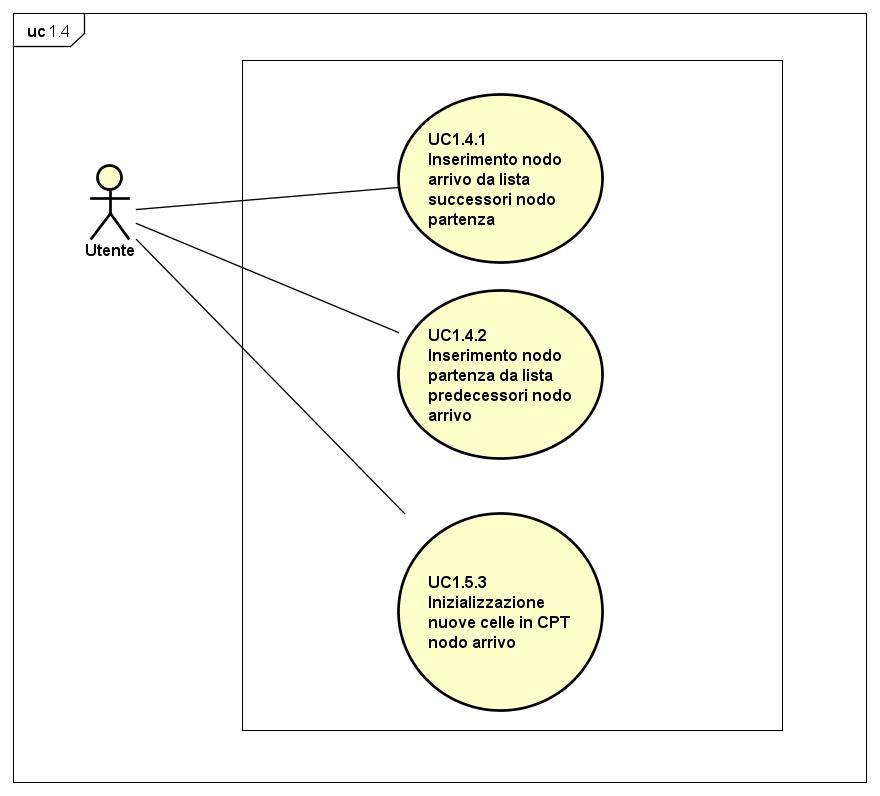
\includegraphics[scale=0.45]{Img/UC1-4} 
	\caption{UC1.4 - Creazione collegamento} \label{} 
\end{figure} 
\begin{itemize} 
	\item{\textbf{Attori primari}: Utente;} 
	\item{\textbf{Scopo e descrizione}: l'attore desidera creare un collegamento tra nodi all'interno della rete. I collegamenti all'interno di una rete Bayesiana sono direzionati, di conseguenza è sempre definito un nodo di partenza ed un nodo d'arrivo;} 
	\item{\textbf{Precondizione}: l'attore ha indicato quale nodi della rete vuole collegare tra loro, qual è il nodo di partenza e qual è il nodo di arrivo;} 
	\item{\textbf{Flusso base degli eventi}: } 
	\begin{itemize} 
		\item{Inserimento nodo arrivo in lista successori del nodo di partenza(UC1.4.1);} 
		\item{Inserimento nodo partenza lista predecessori del nodo di arrivo(UC1.4.2);} 
		\item{Inizializzazione nuove celle in CPT nodo di arrivo(UC1.4.3).} 
	\end{itemize} 
	\item{\textbf{Postcondizione}: il collegamento tra nodi è avvenuto correttamente.} 
\end{itemize} 
\subsection{UC1.4.1: Inserimento nodo arrivo in lista successori del nodo di partenza} 
\hypertarget{UC1.4.1}{} 
\begin{itemize} 
	\item{\textbf{Attori primari}: Utente;} 
	\item{\textbf{Scopo e descrizione}: il nodo di arrivo del collegamento creato viene inserito all'interno della lista dei successori del nodo di partenza;} 
	\item{\textbf{Precondizione}: l'attore ha creato un collegamento tra due nodi;} 
	\item{\textbf{Postcondizione}: l'aggiornamento della lista di successori è avvenuta correttamente.} 
\end{itemize} 
\subsection{UC1.4.2: Inserimento nodo partenza in lista predecessori del nodo di arrivo} 
\hypertarget{UC1.4.2}{} 
\begin{itemize} 
	\item{\textbf{Attori primari}: Utente;} 
	\item{\textbf{Scopo e descrizione}: il nodo di partenza del collegamento creato viene inserito all'interno della lista dei predecessori del nodo di arrivo;} 
	\item{\textbf{Precondizione}: l'attore ha creato un collegamento tra due nodi;} 
	\item{\textbf{Postcondizione}: l'aggiornamento della lista di predecessori è avvenuta correttamente.} 
\end{itemize} 
\subsection{UC1.4.3: Inizializzazione nuove celle in CPT nodo di arrivo} 
\hypertarget{UC1.4.3}{} 
\begin{itemize} 
	\item{\textbf{Attori primari}: Utente;} 
	\item{\textbf{Scopo e descrizione}: in seguito alla creazione di un nuovo collegamento, il nodo di arrivo di quest'ultimo possiede un nuovo predecessore. Di conseguenza esistono nuove possibili combinazioni di stati dei nodi predecessori e di conseguenza nuove celle della CPT;} 
	\item{\textbf{Precondizione}: l'attore ha creato un collegamento tra due nodi;} 
	\item{\textbf{Postcondizione}: le nuove celle della CPT sono state inizializzate con appositi valori di default.} 
\end{itemize} 
\subsection{UC1.5: Eliminazione collegamento} 
\hypertarget{UC1.5}{} 
\begin{figure} [H]
	\centering
	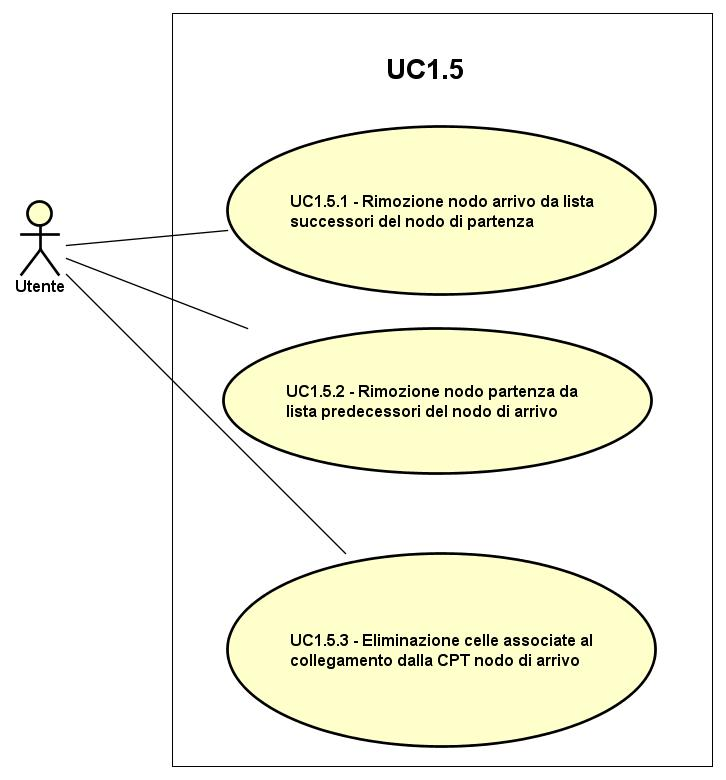
\includegraphics[scale=0.45]{Img/UC1-5} 
	\caption{UC1.5 - Eliminazione collegamento} \label{} 
\end{figure} 
\begin{itemize} 
	\item{\textbf{Attori primari}: Utente;} 
	\item{\textbf{Scopo e descrizione}: l'attore desidera eliminare un collegamento tra nodi all'interno della rete. I collegamenti all'interno di una rete Bayesiana sono direzionati, di conseguenza è sempre definito un nodo di partenza ed un nodo d'arrivo;} 
	\item{\textbf{Precondizione}: l'attore ha indicato quale collegamento vuole eliminare;} 
	\item{\textbf{Flusso base degli eventi}: } 
	\begin{itemize} 
		\item{Rimozione nodo arrivo da lista successori del nodo di partenza(UC1.5.1);} 
		\item{Rimozione nodo partenza da lista predecessori del nodo di arrivo(UC1.5.2);} 
		\item{Eliminazione celle associate al collegamento dalla CPT nodo di arrivo(UC1.5.3).} 
	\end{itemize} 
	\item{\textbf{Postcondizione}: il collegamento tra nodi è stato rimosso correttamente, e le CPT dei successori sono state aggiornate correttamente;} 
\end{itemize} 
\subsection{UC1.5.1: Rimozione nodo arrivo da lista successori del nodo di partenza} 
\hypertarget{UC1.5.1}{} 
\begin{itemize} 
	\item{\textbf{Attori primari}: Utente;} 
	\item{\textbf{Scopo e descrizione}: il nodo di arrivo del collegamento che si vuole eliminare viene rimosso dalla lista dei successori del nodo di partenza;} 
	\item{\textbf{Precondizione}: l'attore ha richiesto l'eliminazione di un collegamento tra due nodi;} 
	\item{\textbf{Postcondizione}: l'aggiornamento della lista di successori del nodo di partenza è avvenuta correttamente.} 
\end{itemize} 
\subsection{UC1.5.2: Rimozione nodo partenza da lista predecessori del nodo di arrivo} 
\hypertarget{UC1.5.2}{} 
\begin{itemize} 
	\item{\textbf{Attori primari}: Utente;} 
	\item{\textbf{Scopo e descrizione}: il nodo di partenza del collegamento che si vuole eliminare viene rimosso dalla lista dei predecessori del nodo di arrivo;} 
	\item{\textbf{Precondizione}: l'attore ha richiesto l'eliminazione di un collegamento tra due nodi;} 
	\item{\textbf{Postcondizione}: l'aggiornamento della lista di predecessori del nodo di arrivo è avvenuta correttamente.} 
\end{itemize} 
\subsection{UC1.5.3: Eliminazione celle associate al collegamento dalla CPT nodo di arrivo} 
\hypertarget{UC1.5.3}{} 
\begin{itemize} 
	\item{\textbf{Attori primari}: Utente;} 
	\item{\textbf{Scopo e descrizione}: in seguito all'eliminazione di un collegamento, il nodo di arrivo di quest'ultimo possiede un predecessore in meno. Di conseguenza esistono meno possibili combinazioni di stati dei nodi predecessori. Tutte le celle della tabella associate al predecessore rimosso devono essere eliminate;} 
	\item{\textbf{Precondizione}: l'attore ha richiesto l'eliminazione di un collegamento tra due nodi;} 
	\item{\textbf{Postcondizione}: le celle in eccesso sono state rimosse correttamente.} 
\end{itemize} 
\subsection{UC1.6: Salvataggio rete} 
\hypertarget{UC1.6}{} 
\begin{itemize} 
	\item{\textbf{Attori primari}: Utente;} 
	\item{\textbf{Scopo e descrizione}: l'intera struttura realizzata dall'utente tramite l'editor grafico, cioè l'insieme dei nodi ed i collegamenti tra essi, deve essere salvabile su disco all'interno di un apposito file JSON;} 
	\item{ \textbf{Precondizione}: l'attore ha indicato al sistema di voler salvare la rete all'interno di un apposito file JSON;} 
	\item{\textbf{Postcondizione}: viene salvato su disco un file JSON contenente la struttura della rete realizzata.} 
\end{itemize} 
\subsection{UC1.7: Errore modifica nodo}
\begin{itemize} 
	\item{\textbf{Attori primari}: Utente;} 
	\item{\textbf{Scopo e descrizione}: l'attore, durante un'operazione di modifica di un nodo, ha inserito dei valori non validi per uno o più parametri. La causa dell'errore dovrà essere opportunamente segnalata all'attore. Il nodo e tutti i collegamenti ad esso associati, fintanto che gli errori non verranno risolti, risulteranno come temporaneamente inattivi all'interno della rete;} 
	\item{\textbf{Precondizione}: l'attore ha eseguito una o più operazioni di modifica ad un nodo inserendo valori non validi;} 
	\item{\textbf{Postcondizione}: gli errori sono stati gestiti correttamente e l'attore è stato informato di essi;} 
\end{itemize}   
\subsection{UC1.8: Salvataggio file JSON} 
\hypertarget{UC1.8}{} 
\begin{figure} [H]
	\centering
	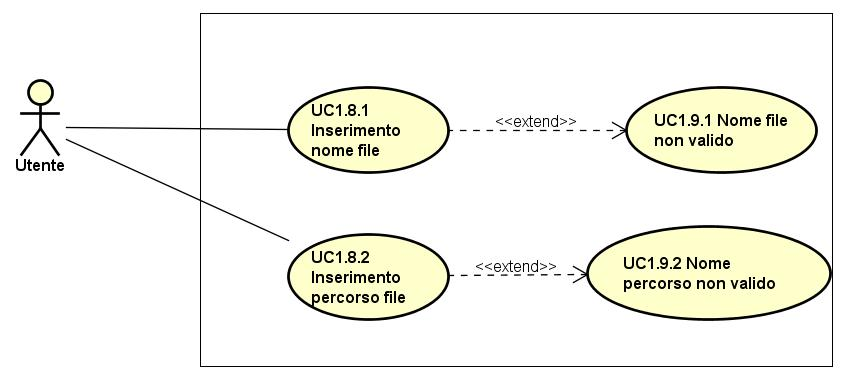
\includegraphics[scale=0.45]{Img/UC1-8} 
	\caption{UC1.8 - Salvataggio file JSON} \label{} 
\end{figure} 
\begin{itemize} 
	\item{\textbf{Attori primari}: Utente;} 
	\item{\textbf{Scopo e descrizione}: l'attore desidera salvare un file JSON, utilizzato per memorizzare diverse impostazioni della rete. Un file JSON è identificato principalmente da due componenti: un nome ed un percorso in cui è salvato all'interno del file system;} 
	\item{\textbf{Precondizione}: l'attore ha indicato di volere salvare la rete su file;} 
	\item{\textbf{Flusso base degli eventi}: } 
	\begin{itemize} 
		\item{L'attore inserisce il nome del file(UC1.8.1);} 
		\item{L'attore inserisce il percorso in cui salvare il file (UC1.8.2).} 
	\end{itemize} 
	\item{\textbf{Postcondizione}: il file è stato salvato correttamente.} 
	\item \textbf{Estensioni}:
	\begin{itemize}
		\item Viene salvato un JSON non valido, il sistema rimane nello stato precedente all'azione informando l'utente dell'accaduto(UC1.9);
	\end{itemize}
\end{itemize} 
\subsection{UC1.8.1: Inserimento nome file} 
\hypertarget{UC1.8.1}{} 
\begin{itemize} 
	\item{\textbf{Attori primari}: Utente;} 
	\item{\textbf{Scopo e descrizione}: l'attore inserisce il nome con cui vuole salvare un file JSON;} 
	\item{\textbf{Precondizione}: l'attore ha indicato di volere salvare il file;} 
	\item{\textbf{Postcondizione}: il file è stato nominato correttamente.} 
\end{itemize} 
\subsection{UC1.8.2: Inserimento percorso file} 
\hypertarget{UC1.8.2}{} 
\begin{itemize} 
	\item{\textbf{Attori primari}: Utente;} 
	\item{\textbf{Scopo e descrizione}: l'attore inserisce il percorso in cui vuole salvare il file associato alla rete;} 
	\item{\textbf{Precondizione}: l'attore ha indicato di volere salvare la rete su file;} 
	\item{\textbf{Postcondizione}: il percorso in cui salvare il file è stato definito correttamente.}
\end{itemize} 
\subsection{UC1.9: Errore salvataggio file JSON} 
\hypertarget{UC1.9}{} 
\begin{itemize} 
	\item{\textbf{Attori primari}: Utente;} 
	\item{\textbf{Scopo e descrizione}:Il salvataggio del file JSON su disco non è terminato con successo, ciò può essere causato da una moltitudine di ragioni, le più comuni possono essere: l'inserimento di un nome non valido, l'inserimento di un percorso non valido, o problemi hardware;} 
	\item{\textbf{Precondizione}: l'attore ha indicato di volere salvare la rete su file;} 
	\item{\textbf{Postcondizione}: Il salvataggio del file JSON non è terminato con successo, e l'utente è stato informato del fallimento dell'operazione.} 
\end{itemize}
